\documentclass[10pt]{article}
\makeatletter
\def\input@path{{tmlr-style/}}
\makeatother
\usepackage[preprint]{tmlr}
\usepackage{booktabs}
\usepackage{amsmath,amssymb}
\usepackage{graphicx}
\usepackage{microtype}
\usepackage{hyperref}
\usepackage{url}

\title{PersonaVoice: One-Second Voice Cloning with Length-Adaptive Flow Matching}

\author{\name Jiang Luchang \\
\addr \texttt{auroral.sunflower@gmail.com} \\
\url{https://orcid.org/0009-0004-4579-4243}}

\hypersetup{
  pdftitle={PersonaVoice: One-Second Voice Cloning with Length-Adaptive Flow Matching},
  pdfauthor={Jiang Luchang},
  pdfsubject={Zenodo preprint},
  pdfkeywords={short-reference voice cloning, text-to-speech, flow matching, F5-TTS, length-adaptive generation, speaker similarity}
}

\begin{document}
\maketitle

\begin{abstract}
Zero-shot voice cloning is usually evaluated with several seconds of reference
speech. We study the more restrictive one-second regime, where a system must
preserve speaker identity while the target text varies from a few words to
multi-sentence utterances. PersonaVoice is a plug-in adaptation of the official
F5-TTS flow-matching path that combines Silero-VAD and RMS reference
normalization, an orthogonal environment submanifold, length-aware chunking,
and dynamic activation of a zero-initialized persona/emotion FiLM adapter. The
design keeps the pretrained flow path as the source of generation and treats
identity, intelligibility, and catastrophic failure as separate endpoints.
On 200 held-out LibriTTS dev-clean utterances with one-second references,
PersonaVoice v10.4.7 obtains ECAPA-TDNN speaker similarity (SECS)
$0.4945\pm0.1800$ and Whisper WER $0.1928\pm0.3077$. It exceeds the measured
XTTS v2 and CosyVoice systems in SECS (0.3349 and 0.3595), while XTTS v2 has
lower WER (0.1296). The aggregate score hides a sharp length effect: WER is
0.1158 for texts longer than eight words but 0.4066 for shorter texts, with a
35.8\% catastrophic-failure rate (WER $>0.5$). Controlled ablations remove
legacy TD-CFG, IBOP, and SBM modules without measurable benefit, motivating the
simplified release configuration. The result is therefore a reproducible
identity--alignment trade-off study, not a claim of universally superior TTS,
validated perceptual persona control, or psychological reconstruction.
\end{abstract}

\section{Introduction}

A one-second reference contains enough acoustic evidence to suggest a speaker,
but too little to make every downstream decision stable. In a zero-shot
text-to-speech system, the same reference can produce a high-similarity sample
whose words are wrong, or intelligible speech whose voice is weakly matched.
This coupling is especially visible when the target text is very short: the
flow-matching model has few text tokens with which to anchor a trajectory, while
the reference still imposes a strong speaker condition.

Recent zero-shot systems such as F5-TTS and VoiceCraft make short-reference
generation practical, but do not remove this evaluation coupling
\citep{chen-etal-2025-f5,peng-etal-2024-voicecraft}. We investigate this regime as a measurement problem rather than a slogan about
``one-second cloning.'' PersonaVoice v10.4.7 is an implementation-oriented
adapter around the official F5-TTS computation path. Its central mechanism,
Length-Aware Adaptive Generation (LAAG), changes the generation unit with text
length: short inputs use a single stable pass, while longer inputs are split
into bounded chunks and cross-faded. An orthogonal environment submanifold
(OES) separates a controllable environment component from the speaker vector,
and a zero-initialized FiLM module provides a plug-in path for persona and
emotion controls without changing the no-control model at initialization.

The paper makes four contributions. First, it defines a one-second reference
benchmark with a fixed 200-item LibriTTS dev-clean evaluation set and reports
both similarity and intelligibility rather than a single score. Second, it
describes an official-path implementation of OES and LAAG, including the
mel-concatenation correction and dynamic FiLM policy used in the released
configuration. Third, it compares the system with XTTS v2, CosyVoice, and the
official F5-TTS baseline under the same reference-duration target. Fourth, it
reports negative ablations and a catastrophic-failure analysis that exposes the
short-text failure mode. We do not claim that the optional persona/emotion
controls recover a person's psychological traits; their perceptual validation
requires a separate listener study.

\begin{figure}[t]
  \centering
  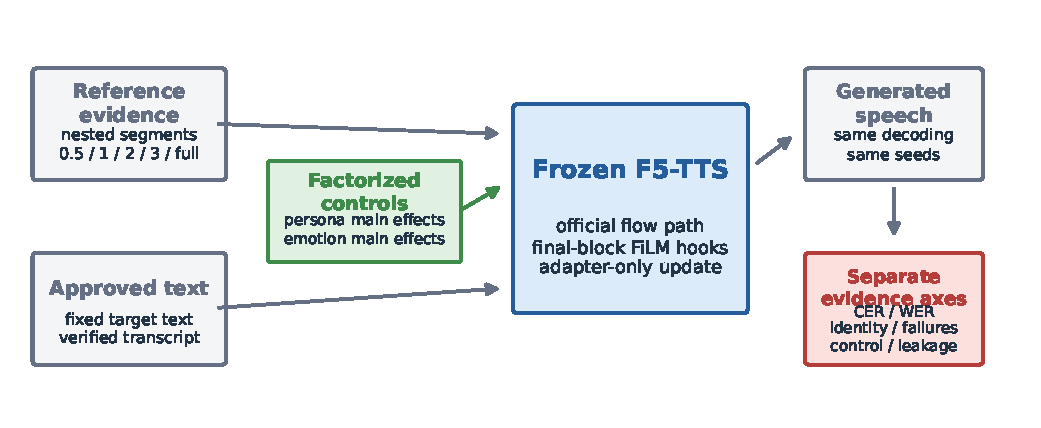
\includegraphics[width=.82\linewidth]{figures/tmlr_speech_overview.pdf}
  \caption{PersonaVoice v10.4.7. A one-second reference is normalized and
  encoded, OES controls the environment component, and LAAG selects a
  single-pass or chunked official F5-TTS flow. The optional FiLM path is
  activated only when a non-zero control is requested and is evaluated here as
  an implementation boundary, not as a psychological measurement.}
  \label{fig:overview}
\end{figure}

\section{System and Implementation}

\subsection{One-second conditioning}

Let $r$ be a waveform and $d=1$ second the reference budget. The front-end
uses Silero VAD to identify voiced material and RMS normalization to reduce
recording-level energy variation. The resulting mel reference is passed to
the official F5-TTS conditional flow path together with the verified reference
transcript. Speaker identity is measured independently with a pinned
ECAPA-TDNN encoder; that encoder is not used as a training target in the
reported benchmark.

\subsection{Orthogonal environment submanifold}

The speaker encoder output $z\in\mathbb{R}^{192}$ can contain both timbre and
recording-environment information. PersonaVoice learns an environment basis
$B\in\mathbb{R}^{192\times32}$ and forms
\begin{equation}
 z_{env}=\sigma_{env}(zB)B^\top, \qquad z_{tim}=z-z_{env},
 \qquad z_{out}=z_{tim}+\omega z_{env}.
\end{equation}
The QR-orthogonalized basis makes the decomposition auditable. The released
configuration uses a small initial environment scale and $\omega=0$ for the
clean-timbre operating point. This is a controllable representation choice,
not a claim that acoustic environments are perfectly separable.

\subsection{Length-Aware Adaptive Generation}

LAAG selects the generation unit from the target text. Text longer than the
configured character budget is split into chunks of at most 135 characters;
each chunk is synthesized with the same one-second reference and then joined
with mel-domain and waveform cross-fades. A dimension-order bug in the mel
splice was corrected in v10.4.5. The current v10.4.7 configuration uses the
official F5 duration computation, 32 integration steps, sway coefficient
$-1.0$, and static CFG 2.5.

The dynamic FiLM policy is length-aware. With a single chunk, FiLM is off by
default to avoid over-correcting short trajectories. With multiple chunks, the
adapter can be activated to anchor the speaker condition across chunks. For a
hidden state $h$, persona $p$, and emotion $e$, the plug-in computes
\begin{equation}
 h'=(1+\lambda\Delta\gamma(p,e))\odot h+\lambda\beta(p,e),
\end{equation}
where both networks are zero-initialized, following the general idea of
conditioning intermediate representations with feature-wise modulation
\citep{perez2018film}. The final two DiT blocks receive
the hooks; the backbone path remains unchanged when $\lambda=0$. This
parameterization makes the controls operationally distinct from the identity
embedding, but the present paper does not treat them as validated personality
or emotion estimators.

\begin{figure}[t]
  \centering
  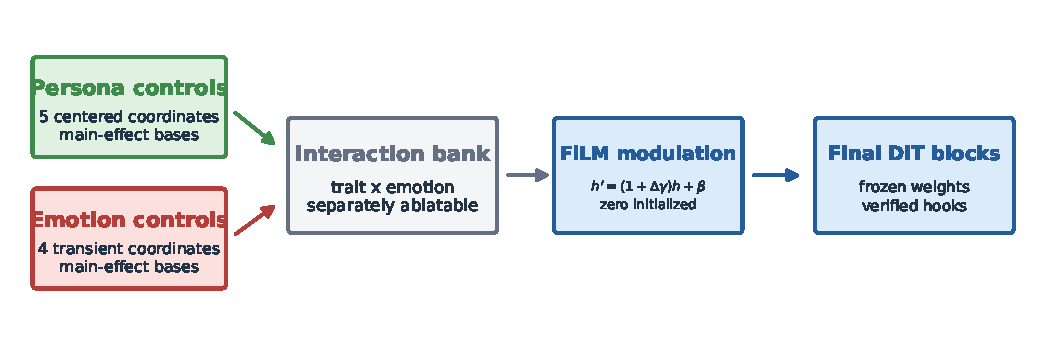
\includegraphics[width=.82\linewidth]{figures/tmlr_film_mechanism.pdf}
  \caption{The FiLM adapter is a zero-initialized, separately addressable
  control path. The reported 200-item benchmark evaluates the identity and
  text endpoints of the release configuration; perceptual control effects are
  outside the measured claims.}
  \label{fig:film}
\end{figure}

\subsection{Removed guidance modules}

The repository retains experimental implementations of temporal-decay CFG,
IBOP, SBM, and cross-entropy attention guidance (CEAG). The final release
disables CEAG and best-of-$N$ sampling because their incremental benefit over
the LAAG plus official-flow baseline was negligible or negative in the
corresponding ablations. Reporting these removals is important: the final
system is a smaller, more stable configuration than the historical prototype.

\section{Experimental Protocol}

\subsection{Data and reference construction}

We evaluate 200 held-out utterances from LibriTTS dev-clean, selected with
seed 42. Each item supplies target text and a one-second reference segment;
the same item list is used for PersonaVoice and external baselines. The
reference duration is fixed before synthesis and no generated sample is used
for model selection. The bundled single-file demo is reported separately and
is not part of the 200-item estimate.

\subsection{Metrics}

Speaker similarity is cosine similarity between ECAPA-TDNN embeddings of the
reference and generated waveform (SECS). Intelligibility is word error rate
from Whisper-large-v3-turbo. We additionally report catastrophic failure rate
(CFR), defined as the fraction of items with WER $>0.5$, and real-time factor
where available. Because SECS and WER measure different properties, all claims
are made on the joint table rather than on a composite score.

\subsection{Baselines and ablations}

The external comparison includes XTTS v2, CosyVoice, and the official F5-TTS
path. The corresponding JSON artifact records 200 successful baseline runs,
the same one-second target, the ECAPA/Whisper evaluation chain, and seed 42.
The final PersonaVoice statistic is the v10.4.7 200-item artifact. The
external runs are reported as protocol-matched comparisons; because the
available baseline artifact is not a paired rerun of every final checkpoint,
we do not attach paired significance tests to cross-system differences.

The internal ablation set removes TD-CFG, IBOP, and SBM one at a time from the
200-item pipeline. Paired tests use the same item IDs. We use two-sided paired
$t$ tests as descriptive diagnostics and retain effect sizes; these ablations
are not presented as a search over test-set configurations.

\begin{figure}[t]
  \centering
  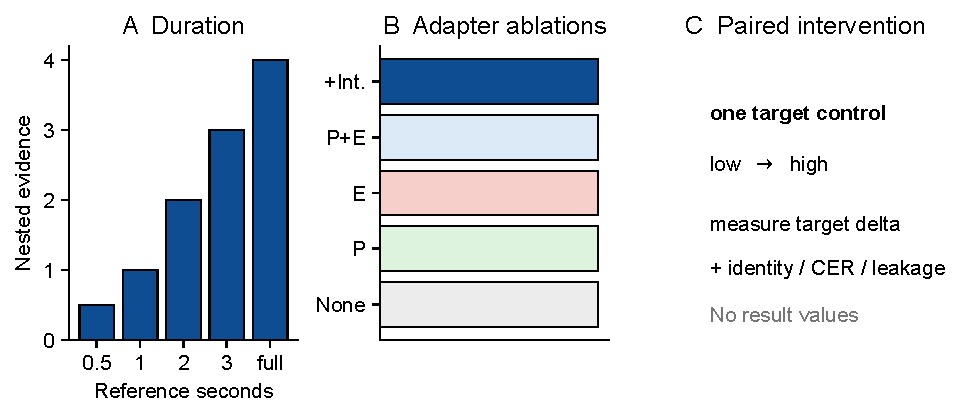
\includegraphics[width=.86\linewidth]{figures/tmlr_evaluation_matrix.pdf}
  \caption{Evaluation matrix. Reference duration and text length are held
  fixed within each comparison; similarity, intelligibility, and failure are
  reported separately.}
  \label{fig:matrix}
\end{figure}

\section{Results}

\subsection{Main one-second comparison}

Table~\ref{tab:main} shows the principal result. PersonaVoice has the highest
measured SECS among the reported systems, but XTTS v2 has the lowest WER. The
result is a trade-off, not a universal ranking: the flow-matching adapter
preserves more speaker evidence while the autoregressive baseline supplies
stronger local text constraints.

\begin{table}[t]
\centering
\small
\begin{tabular}{lccc}
\toprule
System & SECS $\uparrow$ & WER $\downarrow$ & $n$ \\
\midrule
PersonaVoice v10.4.7 & \textbf{0.4945} & 0.1928 & 200 \\
XTTS v2 & 0.3349 & \textbf{0.1296} & 200 \\
CosyVoice & 0.3595 & 0.6130 & 200 \\
Official F5-TTS & 0.2508 & 0.8982 & 200 \\
\bottomrule
\end{tabular}
\caption{One-second reference comparison. PersonaVoice and the external
baselines use the same metric definitions; the available external artifact is
protocol-matched but not a fully paired rerun of every final checkpoint.}
\label{tab:main}
\end{table}

On the 200-item PersonaVoice run, SECS is $0.4945\pm0.1800$ (95\% CI
$[0.4694,0.5196]$) and WER is $0.1928\pm0.3077$ (95\% CI
$[0.1499,0.2358]$). The median values are 0.5226 and 0.0588 respectively,
which already indicate a heavy-tailed failure distribution. CFR is 13.5\%
(27/200), so the mean WER must not be read as a guarantee of usable output.

\subsection{Text-length stratification}

The length curve is the central diagnostic for LAAG. For texts longer than
eight words ($n=147$), SECS is 0.5044 and WER is 0.1158, with CFR 5.4\%. For
texts of eight words or fewer ($n=53$), SECS falls to 0.4671, WER rises to
0.4066, and CFR rises to 35.8\%. The extreme subset of at most four words
contains 22 items, WER 0.6629, and CFR 63.6\%. Thus the aggregate similarity
advantage is compatible with a serious short-text alignment failure.

\begin{table}[t]
\centering
\small
\begin{tabular}{lrrrr}
\toprule
Text group & $n$ & SECS & WER & CFR \\
\midrule
All & 200 & 0.4945 & 0.1928 & 13.5\% \\
$\leq$8 words & 53 & 0.4671 & 0.4066 & 35.8\% \\
$>$8 words & 147 & 0.5044 & 0.1158 & 5.4\% \\
$\leq$4 words & 22 & 0.4282 & 0.6629 & 63.6\% \\
\bottomrule
\end{tabular}
\caption{Length-stratified PersonaVoice results. CFR is WER $>0.5$; it is
reported to prevent the long-text mean from hiding short-text collapse.}
\label{tab:length}
\end{table}

To expose the tail rather than average it away, we recomputed the same frozen
200-item snapshot with four preregistered word-count buckets.  The shortest
bucket (1--3 words) has WER $0.8333$ and CFR $81.25\%$ (13/16), whereas the
longest bucket has WER $0.1109$ and CFR $5.88\%$ (7/119).  The intermediate
9--15-word bucket is already close to the long-text operating regime.  These
are descriptive strata of one held-out list, not a claim that text length is a
causal intervention.  Wilson 95\% intervals for CFR are $[56.99,93.41]$,
$[7.65,31.14]$, $[0.63,17.71]$, and $[2.88,11.65]$ percentage points for
the four buckets respectively; the wide first interval reflects the small
shortest bucket rather than measurement certainty.

\begin{table}[t]
\centering
\small
\begin{tabular}{lrrrr}
\toprule
Words & $n$ & SECS & WER & CFR \\
\midrule
1--3 & 16 & 0.4331 & 0.8333 & 81.25\% \\
4--8 & 37 & 0.4819 & 0.2221 & 16.22\% \\
9--15 & 28 & 0.4547 & 0.1365 & 3.57\% \\
\textgreater15 & 119 & 0.5161 & 0.1109 & 5.88\% \\
\bottomrule
\end{tabular}
\caption{Fine-grained length analysis from the released per-item snapshot.
CFR is WER $>0.5$; all metrics are computed without test-set selection.}
\label{tab:fine-length}
\end{table}

\begin{figure}[t]
  \centering
  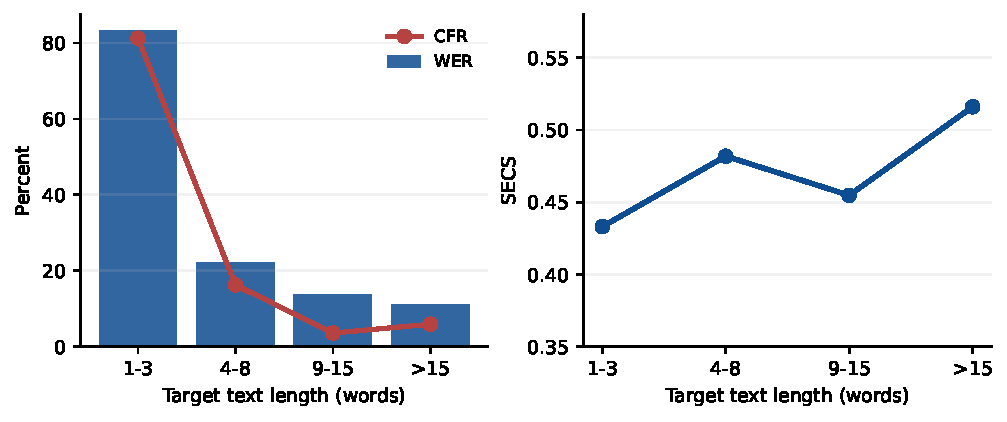
\includegraphics[width=.86\linewidth]{figures/fine_length_curve.pdf}
  \caption{Fine-grained length diagnostic.  The paired WER/CFR view shows a
  sharp short-text failure tail; the SECS panel shows that similarity does not
  provide a corresponding intelligibility guarantee.}
  \label{fig:fine-length}
\end{figure}

\subsection{Ablation results}

Table~\ref{tab:ablation} summarizes the available paired ablations. Removing
TD-CFG changes SECS by $-0.0051$ ($p=.409$, $d=-.058$) and WER by $+0.0030$
($p=.743$, $d=.023$). Removing IBOP changes SECS by $+0.0012$ ($p=.848$,
$d=.014$), while removing SBM changes SECS by $-0.0021$ ($p=.713$,
$d=-.026$). None has a practically meaningful effect in this evaluation.
These results support removal from the release configuration; they do not
prove that the modules are ineffective on every data distribution.

\begin{table}[t]
\centering
\small
\begin{tabular}{lrrr}
\toprule
Ablation & SECS mean & WER mean & SECS $p$ \\
\midrule
Full v8 diagnostic & 0.3774 & 0.2001 & -- \\
Remove TD-CFG & 0.3825 & 0.1971 & .409 \\
Remove IBOP & 0.3762 & 0.1943 & .848 \\
Remove SBM & 0.3795 & 0.1988 & .713 \\
\bottomrule
\end{tabular}
\caption{Paired internal ablations from the repository artifact. The full v8
diagnostic is an historical ablation reference, not the final v10.4.7 main
result; this distinction prevents version mixing.}
\label{tab:ablation}
\end{table}

\subsection{Failure analysis}

The failures are not a smooth degradation. In the 22-item ultra-short group,
five samples have WER 0, while 13 have WER above 0.8. Some failure samples
retain high speaker similarity; for example, the archived `seventeen
seventeen.' case has SECS 0.822 with WER 1.0. This is a consequential failure
mode for voice cloning: a sample can sound like the reference while not saying
the requested words. We therefore treat CFR and per-item records as primary
artifact outputs, rather than selecting audio examples by similarity alone.

The repository also contains a controlled experiment in which Best-of-$N$ and
stronger CFG were applied to ultra-short text. The setting increased WER from
0.4047 to 0.6964 and CFR from 35.8\% to 70.0\% on the tested subset, so it was
removed. This negative result motivates future work on a text-conditioned
alignment mechanism rather than more aggressive sampling.

\begin{figure}[t]
  \centering
  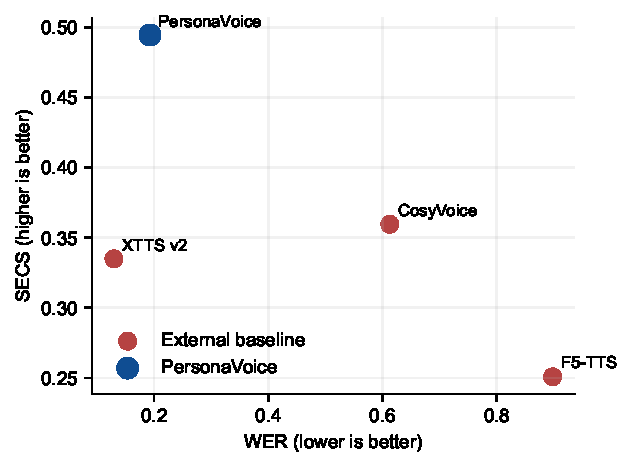
\includegraphics[width=.78\linewidth]{figures/secs_wer_tradeoff.pdf}
  \caption{Joint objective view of the one-second comparison. PersonaVoice
  occupies a high-SECS, moderate-WER point; XTTS v2 has lower WER but lower
  measured similarity. The axes are deliberately not collapsed into a single
  score.}
  \label{fig:secs-wer-tradeoff}
\end{figure}

\begin{figure}[t]
  \centering
  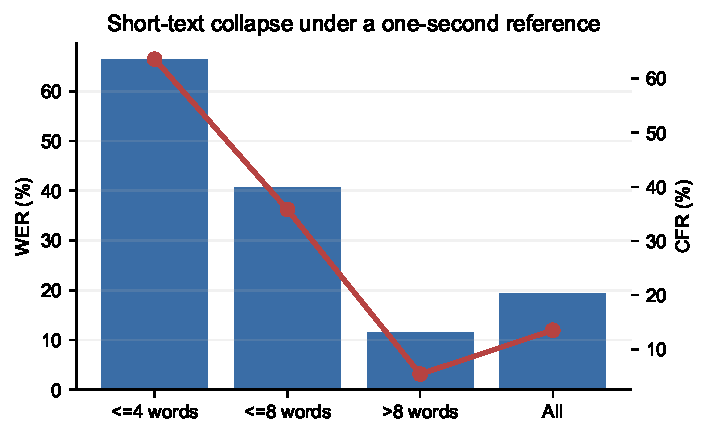
\includegraphics[width=.78\linewidth]{figures/length_failure_curve.pdf}
  \caption{Length-stratified failure curve. The short-text groups expose the
  catastrophic tail hidden by the all-item mean: CFR is 63.6\% for at most four
  words and 35.8\% for at most eight words, versus 5.4\% for longer text.}
  \label{fig:length-failure}
\end{figure}

\section{Reproducibility and Scope}

The release pins the configuration, model identifiers, evaluator names,
reference duration, seed, and per-item JSON rows. Checkpoints and large model
weights are not redistributed. Reproduction requires the licenses and model
downloads documented in the repository. The results are limited to English
LibriTTS dev-clean, a one-second reference budget, and the stated evaluation
pipeline. ECAPA similarity is an objective proxy and does not replace human
similarity judgments; Whisper WER can be biased by language, pronunciation,
and transcript normalization.

The standalone short-reference supplement recomputes the aggregate table,
length curve, fine length buckets, baseline comparison, ablation summary, and
catastrophic-failure ledger from public JSON snapshots. It intentionally
excludes the historical inference implementation, model weights, and audio
files; the snapshots are sufficient to audit the reported numerical claims
without implying a redistributable voice-cloning service. A separate
\texttt{extension\_manifest.json} freezes the planned 0.5/1/2/3-second duration grid
and LAAG/OES ablations. Those condition-level runs are marked pending and are
not used in any table or claim in this preprint.

Code, frozen per-item predictions, and SHA-256 manifests for this version are
available in the
\href{https://github.com/FinalSunFlower/PersonaVoice/tree/paper-supplement-v1.0}{paper-supplement-v1.0 GitHub snapshot}.
The exact artifact snapshot corresponding to this preprint is tagged
\texttt{paper-speech-v1.0}.

The persona extractor and FiLM hooks make the architecture extensible to
style and emotion controls, related to prior controllable speech work
\citep{wang2018style,xie-etal-2025-towards}, but this paper does not claim that the measured
200-item run validates those controls perceptually. A future study must use
paired listener ratings, speaker-level splits, non-target leakage tests, and
ethics review before describing them as effective persona or emotion
interventions.

\section{Broader Impact and Responsible Use}

One-second voice cloning lowers the amount of biometric evidence needed to
imitate a speaker. It can enable fraud, harassment, reputational harm, and
non-consensual synthetic media. The repository therefore treats the system as
a research prototype, requires synthetic-output disclosure, and does not grant
rights to a person's voice or likeness. The measured SECS advantage should not
be interpreted as authorization to impersonate a living or deceased person.

\section{Conclusion}

PersonaVoice demonstrates a reproducible and sharply bounded result in the
extreme short-reference regime. Its official-flow adapter and length-aware
generation achieve strong objective speaker similarity on 200 one-second
conditions, while the same experiments expose a substantial short-text
alignment failure and a clear similarity--WER trade-off. The most useful
contribution is therefore diagnostic: high voice similarity is not sufficient
for reliable speech, and catastrophic text failures must be reported beside
the headline similarity score. The repository's persona/emotion control path
is a foundation for follow-up perceptual work, not evidence of recovered human
personality.

\bibliography{personavoice}
\bibliographystyle{tmlr-style/tmlr}

\appendix
\section{Artifact record}

The release snapshot records the 200-item protocol, aggregate SECS/WER
statistics, length strata, evaluator revisions, and status counts. The
published v10.4.7 values are recomputed from the frozen honest-metrics
snapshot; the external baseline record separately identifies successful runs
and the protocol-matched reference duration. Per-item audio and transcripts
are intentionally not redistributed.

\end{document}
